\documentclass[12pt]{article}

%% Language and font encodings
\usepackage[english]{babel}
\usepackage{multirow}

%% Sets page size and margins
\usepackage[a4paper,top=3cm,bottom=2cm,left=3cm,right=3cm,marginparwidth=1.75cm]{geometry}

%% Useful packages
\usepackage{graphicx}
\usepackage[colorlinks=true, allcolors=blue]{hyperref}
\usepackage{setspace}   %Allows double spacing with the \doublespacing command
\usepackage{indentfirst}

\title{Askie Forum}
\author{
         Danh Nguyen\\
         \texttt{Onid:nguydanh}\\
         \texttt{nguydanh@oregonstate.edu}
         \and
         Joshua Bell\\
         \texttt{Onid:belljos}\\
         \texttt{belljos@oregonstate.edu}
         \and
         Cameron Kocher\\
         \texttt{Onid:kochecam}\\
         \texttt{kochecam@oregonstate.edu}
         \and
         Nicholas Newell\\
         \texttt{Onid:newelln}\\
         \texttt{newelln@oregonstate.edu}
         \and
         Andrew Morrill\\
         \texttt{Onid:morrilan}\\
         \texttt{morrilan@oregonstate.edu}
         \and
         GitHub: https://github.com/hydra314/AskieForum
    }

\begin{document}
\maketitle

\tableofcontents
\section{User Stories:}
\textbf{User Story \#1}
\begin{flushleft}
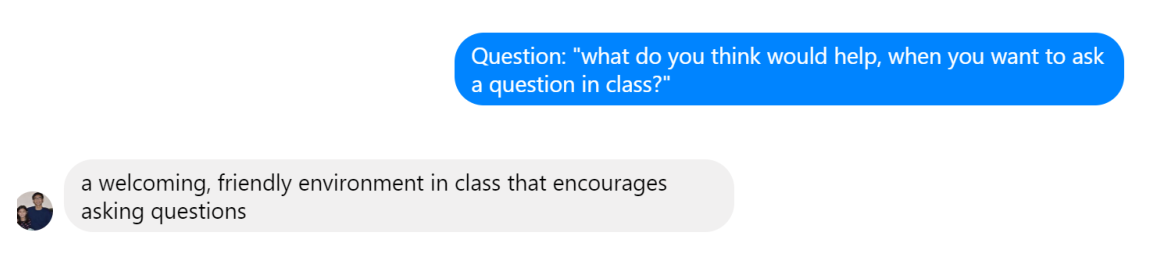
\includegraphics[width=\textwidth]{Assignment5_userstory_1.eps}
\textbf{Description:} Our first user story is from Minh-Tri Tran, a client we obtained through Facebook. There we asked him about what he thinks would help a person ask questions in class. The response we got from him was pretty similar to what we as a team have predicted and mainly focus on. Base on this respond, we will use our team main focus and approach other customer with more compartmentalize questions.\newline
\end{flushleft}

\textbf{User Story \#2}
\begin{flushleft}
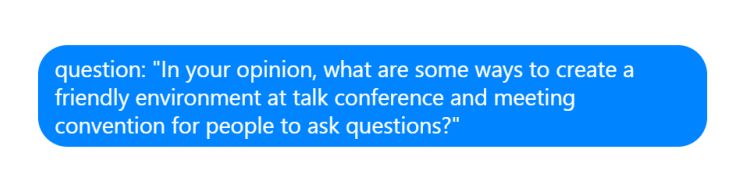
\includegraphics[width=\textwidth]{Assignment5_userstory_2a.eps}
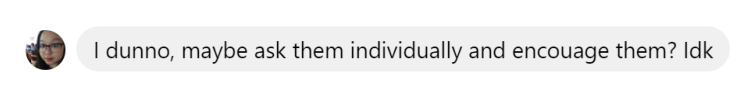
\includegraphics[width=\textwidth]{Assignment5_userstory_2b.eps}
\textbf{Description:} Our next client name is Thu Hoang, she was also a client we obtained through Facebook. From our main approach we asked Thu "what are some ways she thinks would create friendly environment at talk conference and meeting convention?". From her respond above we can see that she mistakenly understood the question and thought that the question was asking about how to make students more comfortable with answering questions rather asking the question. Therefore, we rephrase our question under the same idea for our next user story.\newline
\end{flushleft}

\textbf{User Story \#3}
\begin{flushleft}
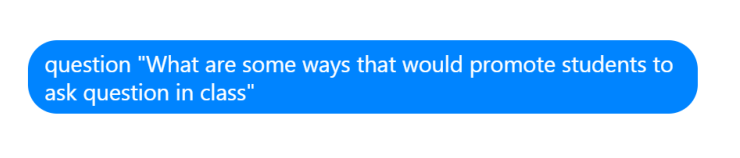
\includegraphics[width=\textwidth]{Assignment5_userstory_3a.eps}
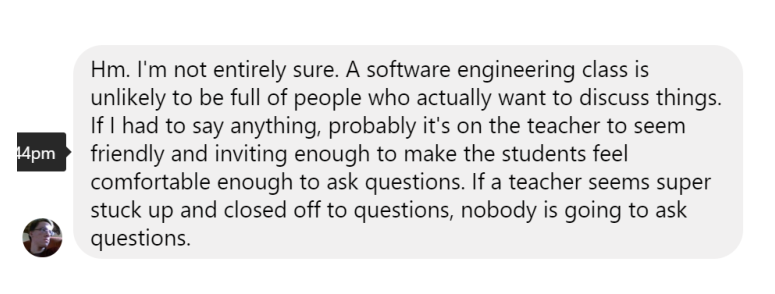
\includegraphics[width=\textwidth]{Assignment5_userstory_3b.eps}
\textbf{Description:} Our third client is Drake and was also obtained from Facebook. As mentioned above we have rephrase our question for Drake under the same approach we had from the start. From his response we see that he isn't giving us any compartmentalize solutions, instead his answer are involve around the process of how people can solve an issues. However, this is not the information we want to obtain since we of course already know that if everyone acted the same way as the theoretical person he just described, then we wouldn't have had an issue with asking questions. What we are really looking for is a solution that involves the usage of a component or a thing that will improve the process of asking question. Therefore we will once again rephrase the question for our client.\newline
\end{flushleft}

\textbf{User Story \#4}
\begin{flushleft}
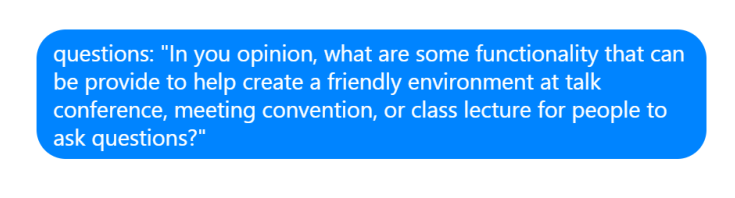
\includegraphics[width=\textwidth]{Assignment5_userstory_4a.eps}
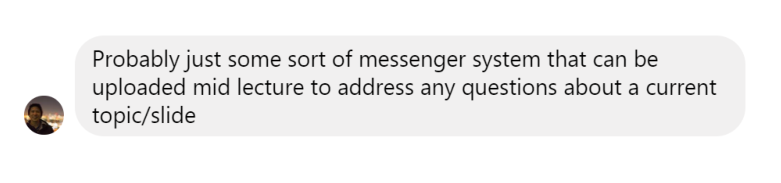
\includegraphics[width=\textwidth]{Assignment5_userstory_4b.eps}
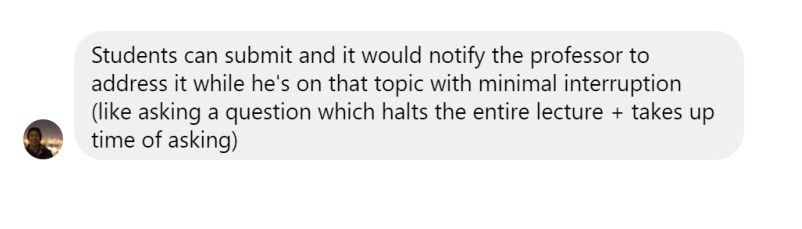
\includegraphics[width=\textwidth]{Assignment5_userstory_4c.eps}
\textbf{Description:} Our next client is Austin, a client we also obtained through Facebook. As you can see above, we have rephrase the questions as describe above. This time we make it more specific to our client that we a looking for a functionality rather than a action. From Austin response, we see that the user are looking for away to ask questions without disrupting the environment. This is useful since he's helping our team validate the usefulness of having a software such as Askie Forum that will allow attendees such as students, or people at meeting conventions to ask questions with minimal interruption.\newline
\end{flushleft}

\textbf{User Story \#5}
\begin{flushleft}
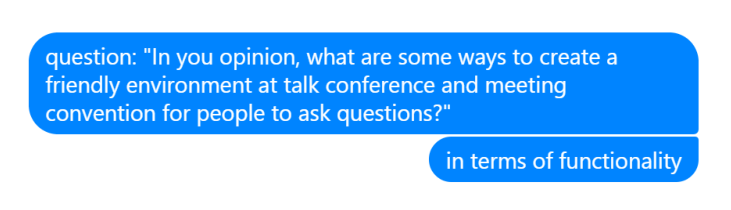
\includegraphics[width=\textwidth]{Assignment5_userstory_5a.eps}
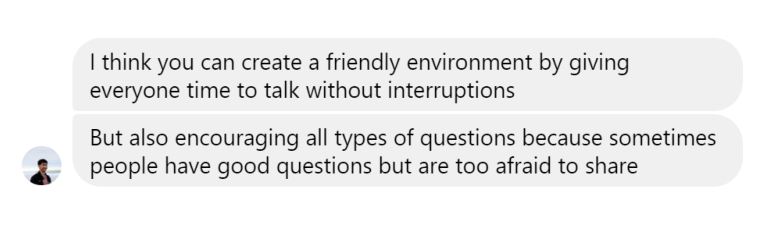
\includegraphics[width=\textwidth]{Assignment5_userstory_5b.eps}
\textbf{Description:} Our next client is Minh To, whom we obtained through Facebook. We asked Minh similarly to Austin about the functionality that can be provided, and his response were really general and very similar to Thu Hoang, and Drake. Therefore, on our next client we will give an example of a functionality that will help them provide an idea that we can use to implement.\newline
\end{flushleft}

\textbf{User Story \#6}
\begin{flushleft}
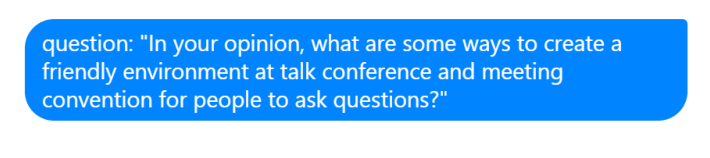
\includegraphics[width=\textwidth]{Assignment5_userstory_6a.eps}
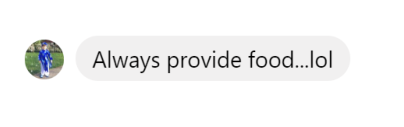
\includegraphics[width=\textwidth]{Assignment5_userstory_6b.eps}
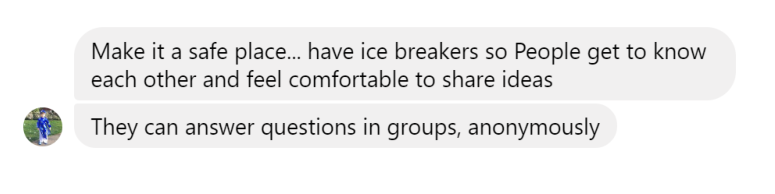
\includegraphics[width=\textwidth]{Assignment5_userstory_6c.eps}
\textbf{Description:} Client \#6 is Yen Nguyen, whom we obtained through Facebook as well. As mentioned above we also asked Yen about the functionality that would help create a better environment for people to ask questions. Based on her response, she's proposing a functionality where each user can have a biography about themselves. This biography will help other user identify someone who can help them obtain a better solution about a certain questions. Because this functionality involves the ability for user to ask other questions individually. Therefore, we will have to obtain a component for our user to do that specific task.\vspace{2cm}
\end{flushleft}

\textbf{User Story \#7}
\begin{flushleft}
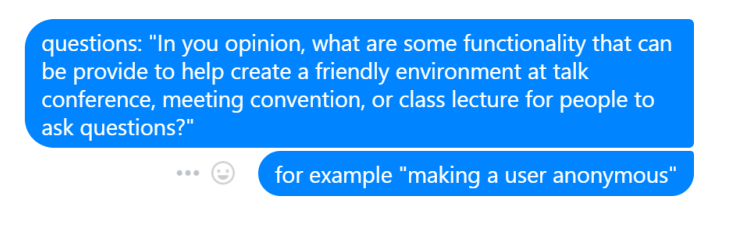
\includegraphics[width=\textwidth]{Assignment5_userstory_7a.eps}
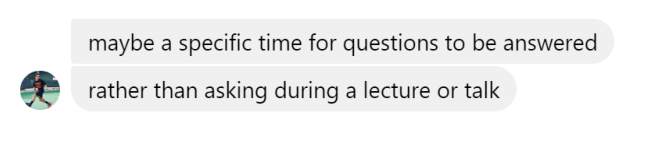
\includegraphics[width=\textwidth]{Assignment5_userstory_7b.eps}
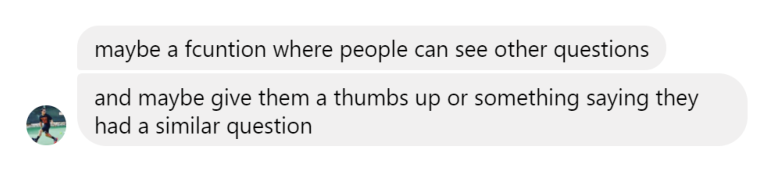
\includegraphics[width=\textwidth]{Assignment5_userstory_7c.eps}
\textbf{Description:} Our 7th client is Ryan Chin also obtained from Facebook. From Ryan's response above we see that we really like the idea of having the user anonymous. He also proposed a really cool function that will allow user to like a question from another user with a thumbs up indicating that they also have a similar question or that they think that it would be really helpful to have that questions answer.\newline
\end{flushleft}

\textbf{User Story \#8}
\begin{flushleft}
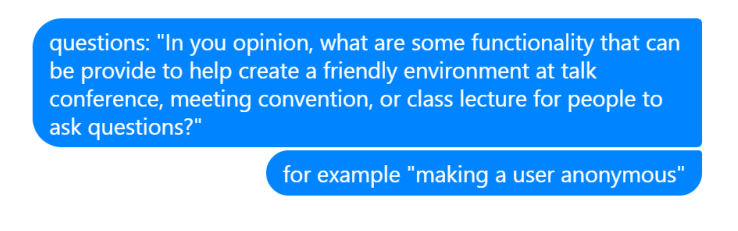
\includegraphics[width=\textwidth]{Assignment5_userstory_8a.eps}
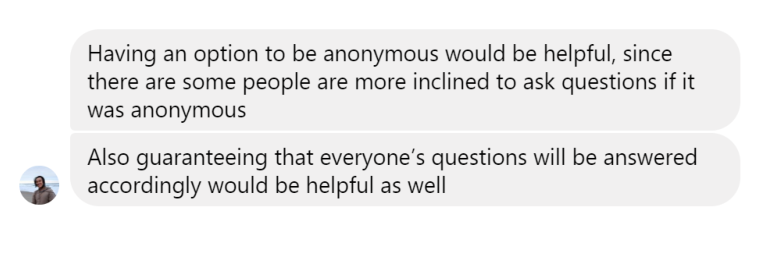
\includegraphics[width=\textwidth]{Assignment5_userstory_8b.eps}
\textbf{Description:} Our client \#8 is Kenny Nguyen, whom we obtained through Facebook. Kenny solutions is very similar to all of the proposed functionality we have already thought of, therefore, it's not something we can use to implement; however, it is more of validating our purpose.\newline
\end{flushleft}

\textbf{User Story \#9}
\begin{flushleft}
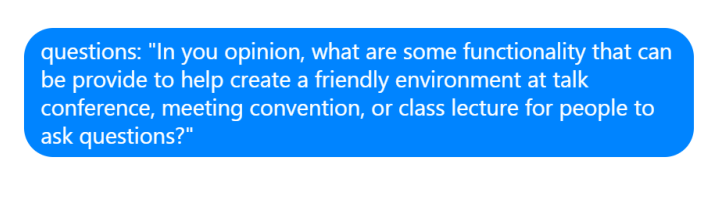
\includegraphics[width=\textwidth]{Assignment5_userstory_9a.eps}
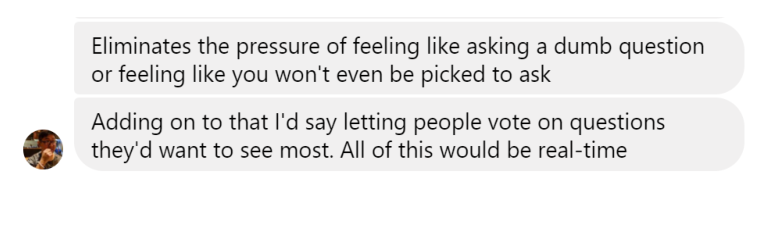
\includegraphics[width=\textwidth]{Assignment5_userstory_9b.eps}
\textbf{Description:} Our client \#9 is Ron, he was also a client we obtained from Facebook. Based on the response we got from Ron, we see that his propose solution are pretty useless since users don't really need to pick out the questions they want to see. Therefore, his response will only be recorded. \newline
\end{flushleft}

\textbf{User Story \#10}
\begin{flushleft}
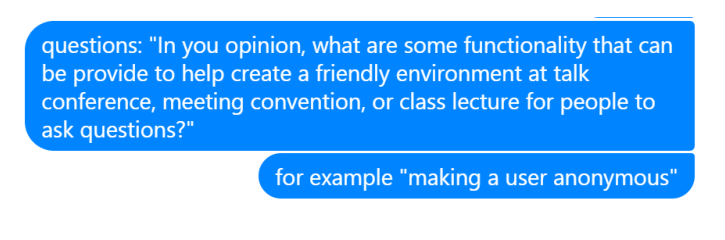
\includegraphics[width=\textwidth]{Assignment5_userstory_10a.eps}
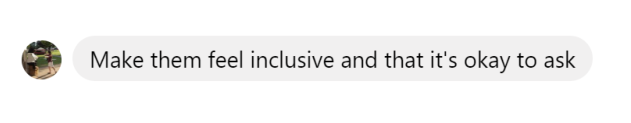
\includegraphics[width=\textwidth]{Assignment5_userstory_10b.eps}
\textbf{Description:} Our next client is Thuy, whom we obtained from Facebook. Thuy response is very similar to Thu Hoang, Drake, and Minh To. Their response where similar because it focus more in terms of the actions rather than functionality; therefore, it is not relevant. \newline
\end{flushleft}

\textbf{User Story \#11}
\begin{flushleft}
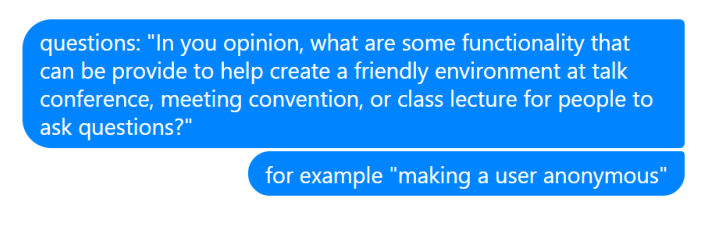
\includegraphics[width=\textwidth]{Assignment5_userstory_11a.eps}
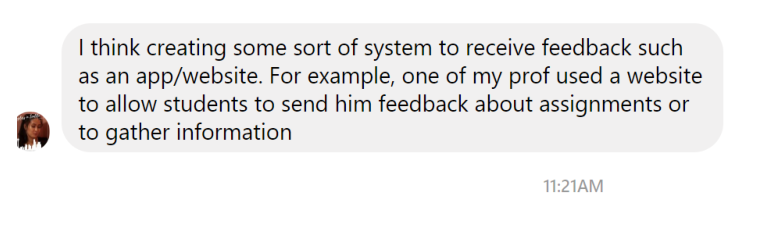
\includegraphics[width=\textwidth]{Assignment5_userstory_11b.eps}
\textbf{Description:} Our very last client is Jody, she is a client we obtained from Facebook. Jody solution is to have a feedback software that will allow people to receive feedback on their assignments. This could be a useful features for teachers whom would like to use their forum as a place to uploaded feedback such as solution on their assignments. \newline
\end{flushleft}

\textbf{Conclusion:} Based on all the user stories we obtained above, we see that Story \#6, \#7, and \#11 are the most essential, because it provides information about some functionality that we can implement to add onto the features that our application can provide to the users. 

\section{Corresponding Tasks:}
\textbf{User Story \#1}
\begin{flushleft}
Implementing a welcoming, friendly environment in class that encourages students to ask questions is more of an end goal for our team than anything else. While we can implement features that will help foster a welcoming environment, the community itself will be responsible for whether or not this is achieved. As such, it's difficult to assign an exact due date for this user story. A specialized user interface and instructor-accessible moderation tools will allow for the creation and maintenance of a friendly classroom environment, but these are features that will be added in later on in the product's development cycle as they are not entirely essential. This task would likely take a pair of programmers no more than a week to complete.
\newline
\end{flushleft}

\textbf{User Story \#2}
\begin{flushleft}
As the question was misunderstood by the customer, this user story is not very useful. The tasks that our team will have to complete for this user story are identical to the ones discussed in the corresponding tasks for User Story \#1: a nice interface for users and a forum moderation toolset for forum hosts. As mentioned before, this would ideally take a pair of programmers less than a week to implement.
\newline
\end{flushleft}

\textbf{User Story \#3}
\begin{flushleft}
Like the first two user stories, this user story focuses on the community of the forum rather than the software used to build it. As such, there is no clear due date; again, the features discussed in the corresponding tasks for User Story \#1 can be implemented to aid in fostering a community that invites students to ask questions.
\newline
\end{flushleft}

\textbf{User Story \#4}
\begin{flushleft}
A messenger system would be a useful addition to Askie Forum, and would be added relatively early into the agile development cycle. Once the essentials - such as the database, basic site functionality, and a basic user interface - are added, a messenger system would follow close behind. Implementing a messenger system would be as simple as extending basic post functionality, and would likely take a pair of programmers about a day or two to complete.
\newline
\end{flushleft}

\textbf{User Story \#5}
\begin{flushleft}
This user story was very similar to the first two, as the customer addressed the community side rather than the software side of Askie Forum. The tasks and due dates for this type of user story were discussed in the corresponding task for User Story \#1.
\newline
\end{flushleft}

\textbf{User Story \#6}
\begin{flushleft}
A biography function would be a useful addition to users' profile pages, and would take very little time to implement. As our team is already planning on implementing user profile pages as a core part of Askie Forum, allowing for an extra input for personal details would be quite easy and could be done alongside the development of user profile pages. User anonymity is also a basic function that we plan to implement. The functionalities mentioned in this user story would therefore be created early into the development cycle, and may be started on as soon as work on the database is completed. A personal information section on user profiles would take about a day to implement, while anonymity may take up to a week.
\newline
\end{flushleft}

\textbf{User Story \#7}
\begin{flushleft}
A thumbs-up feature for questions posted by others would be among the finishing touches and would be implemented late into the development cycle. Having a specific time for questions to be answered would be useful in some scenarios, such as if a professor wanted to lecture for the first half of the class and field questions for the second half. Anonymity was discussed earlier and does not need to be addressed again. Giving users the ability to vote on others' posts (a functionality implemented on popular sites such as Facebook and Reddit) would require a working database, a usable user interface, and a functional posting system; as such, it would be pushed toward the end of the development cycle and would be started on only once the core features have been completed. It would likely take a pair of programmers about half a week to implement. Allowing the forum host to set a time where questions may and may not be asked would also be among the finishing touches put on the product, and would be left until after all the major features have been created. It would take a pair of programmers very little time to implement, as they'd simply have to modify user posting permissions - a feature that should already exist and be modifiable. 
\newline
\end{flushleft}

\textbf{User Story \#8}
\begin{flushleft}
This user story discusses user anonymity, which has already been discussed in the corresponding task for User Story \#6.
\newline
\end{flushleft}

\textbf{User Story \#9}
\begin{flushleft}
Voting on questions was discussed in the corresponding task for User Story \#7. As the description for this user story states, the other half of the response is essentially useless in the context of Askie Forum and will therefore not be considered.
\newline
\end{flushleft}

\textbf{User Story \#10}
\begin{flushleft}
This user story is very similar to ones discussed before, such as User Story \#1 and User Story \#3. The same tasks and due dates apply.
\newline
\end{flushleft}

\textbf{User Story \#11}
\begin{flushleft}
A feedback system would be useful to students and teachers alike. Students would be able to get feedback on their assignments from their teachers, and teachers would be able to receive feedback on their teaching methods and whether or not their assignments were helpful. This would be relatively simple to implement, and could be created once basic posting is functional. It would likely take a pair of programmers about a week to implement.
\newline
\end{flushleft}


\section{UML Sequence Diagram/Spike (20points) (approx 3 pages)}
\begin{flushleft}
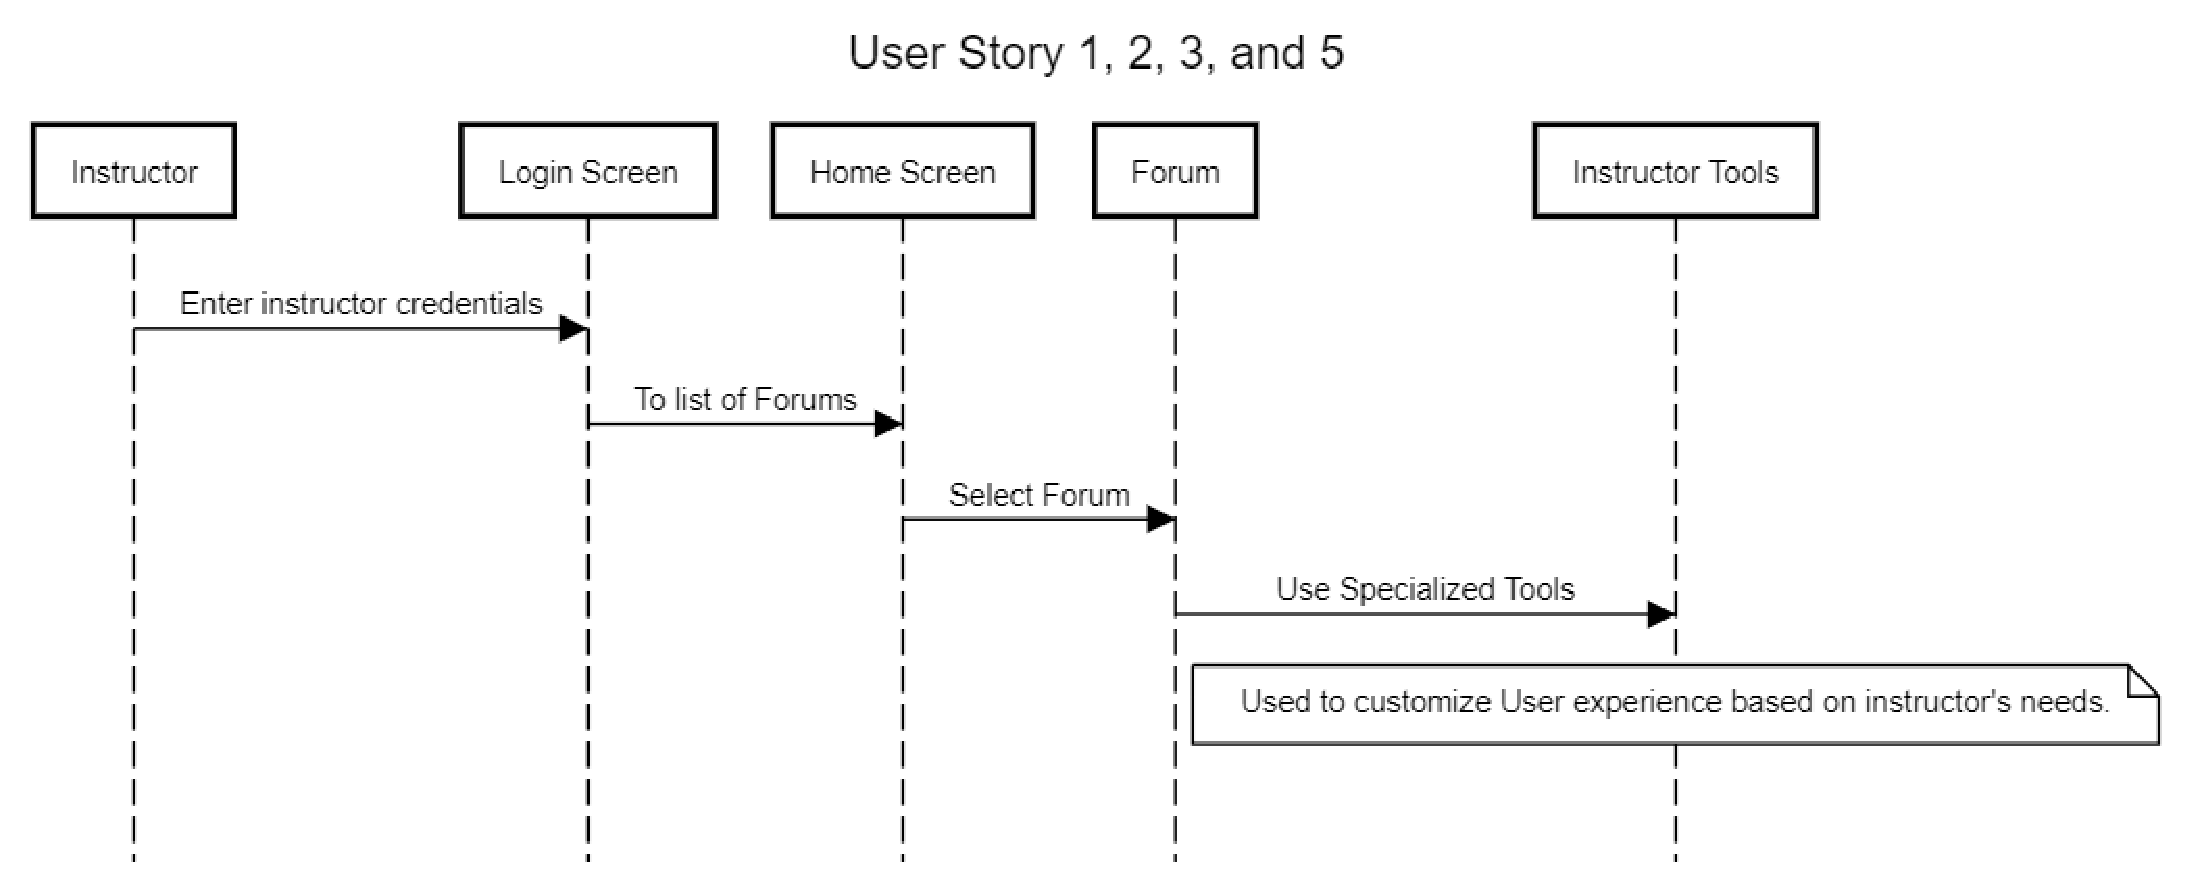
\includegraphics[width=\textwidth]{User_Story_1_2_3_and_5.eps}
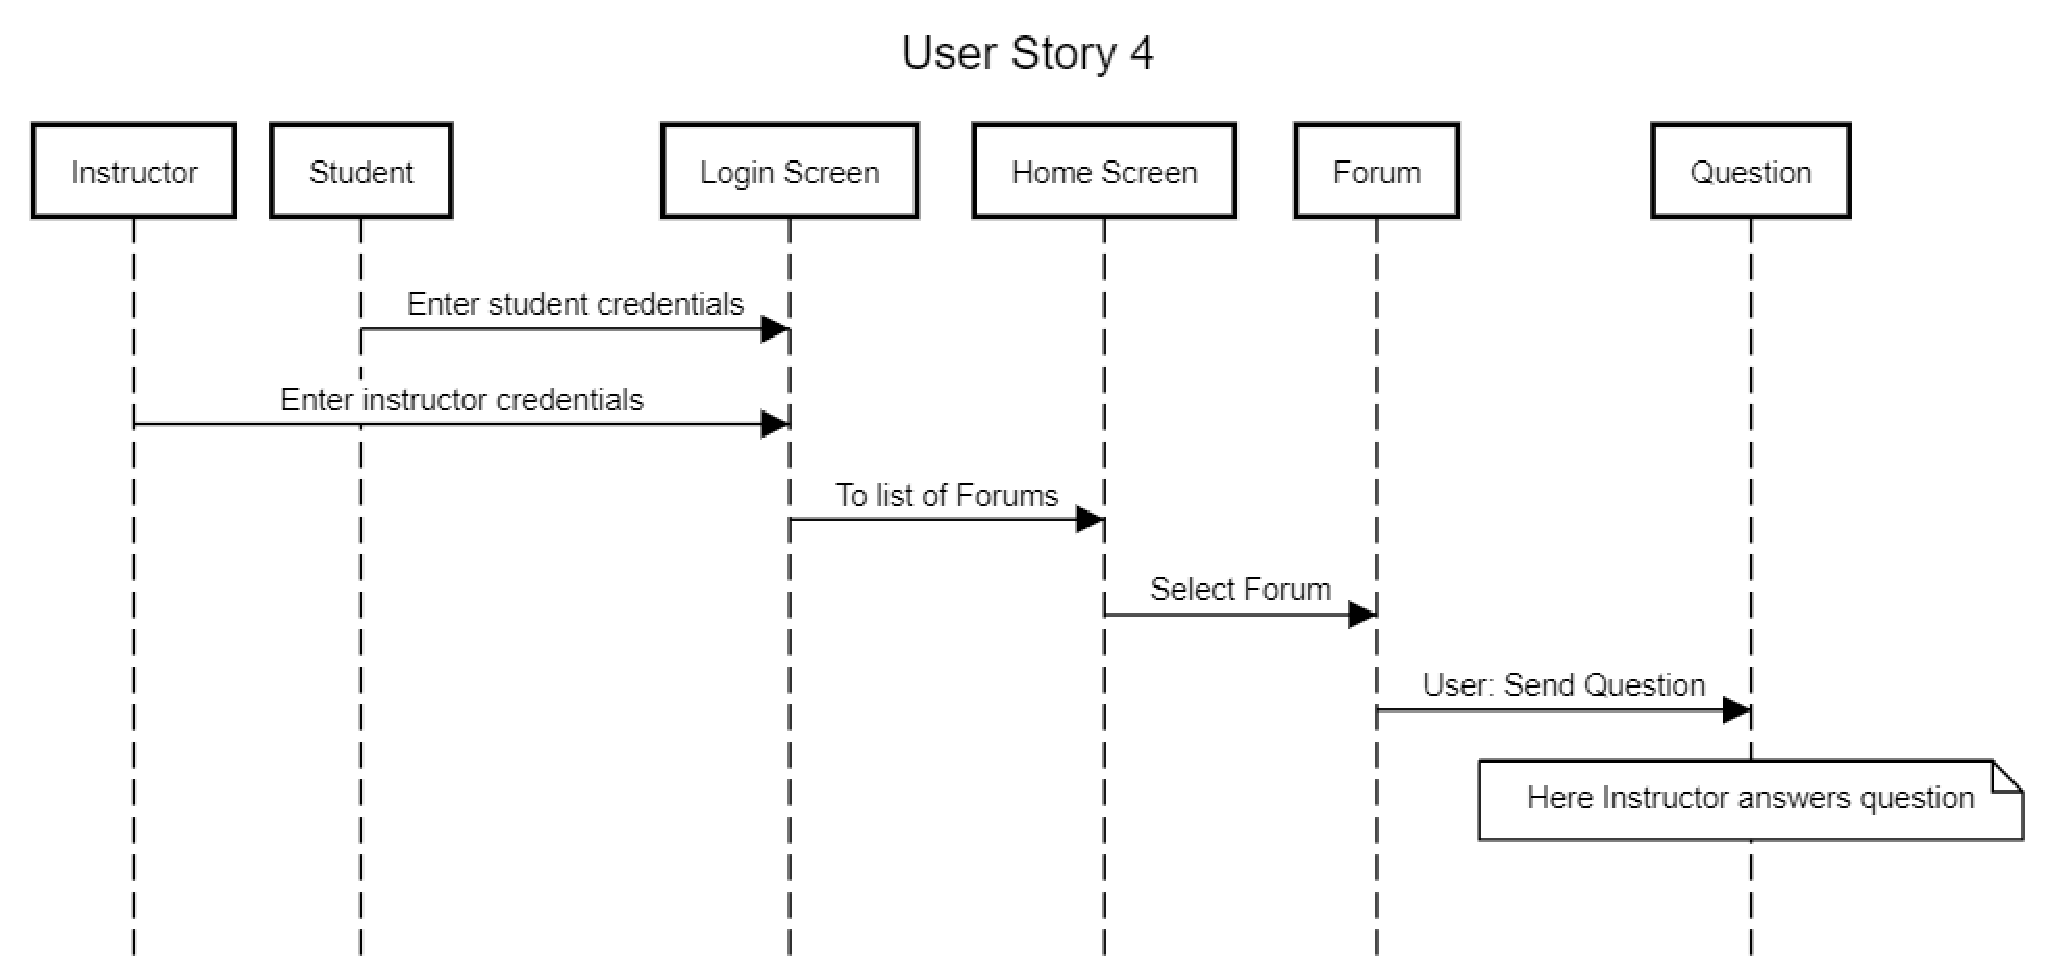
\includegraphics[width=\textwidth]{User_Story_4_SD.eps}
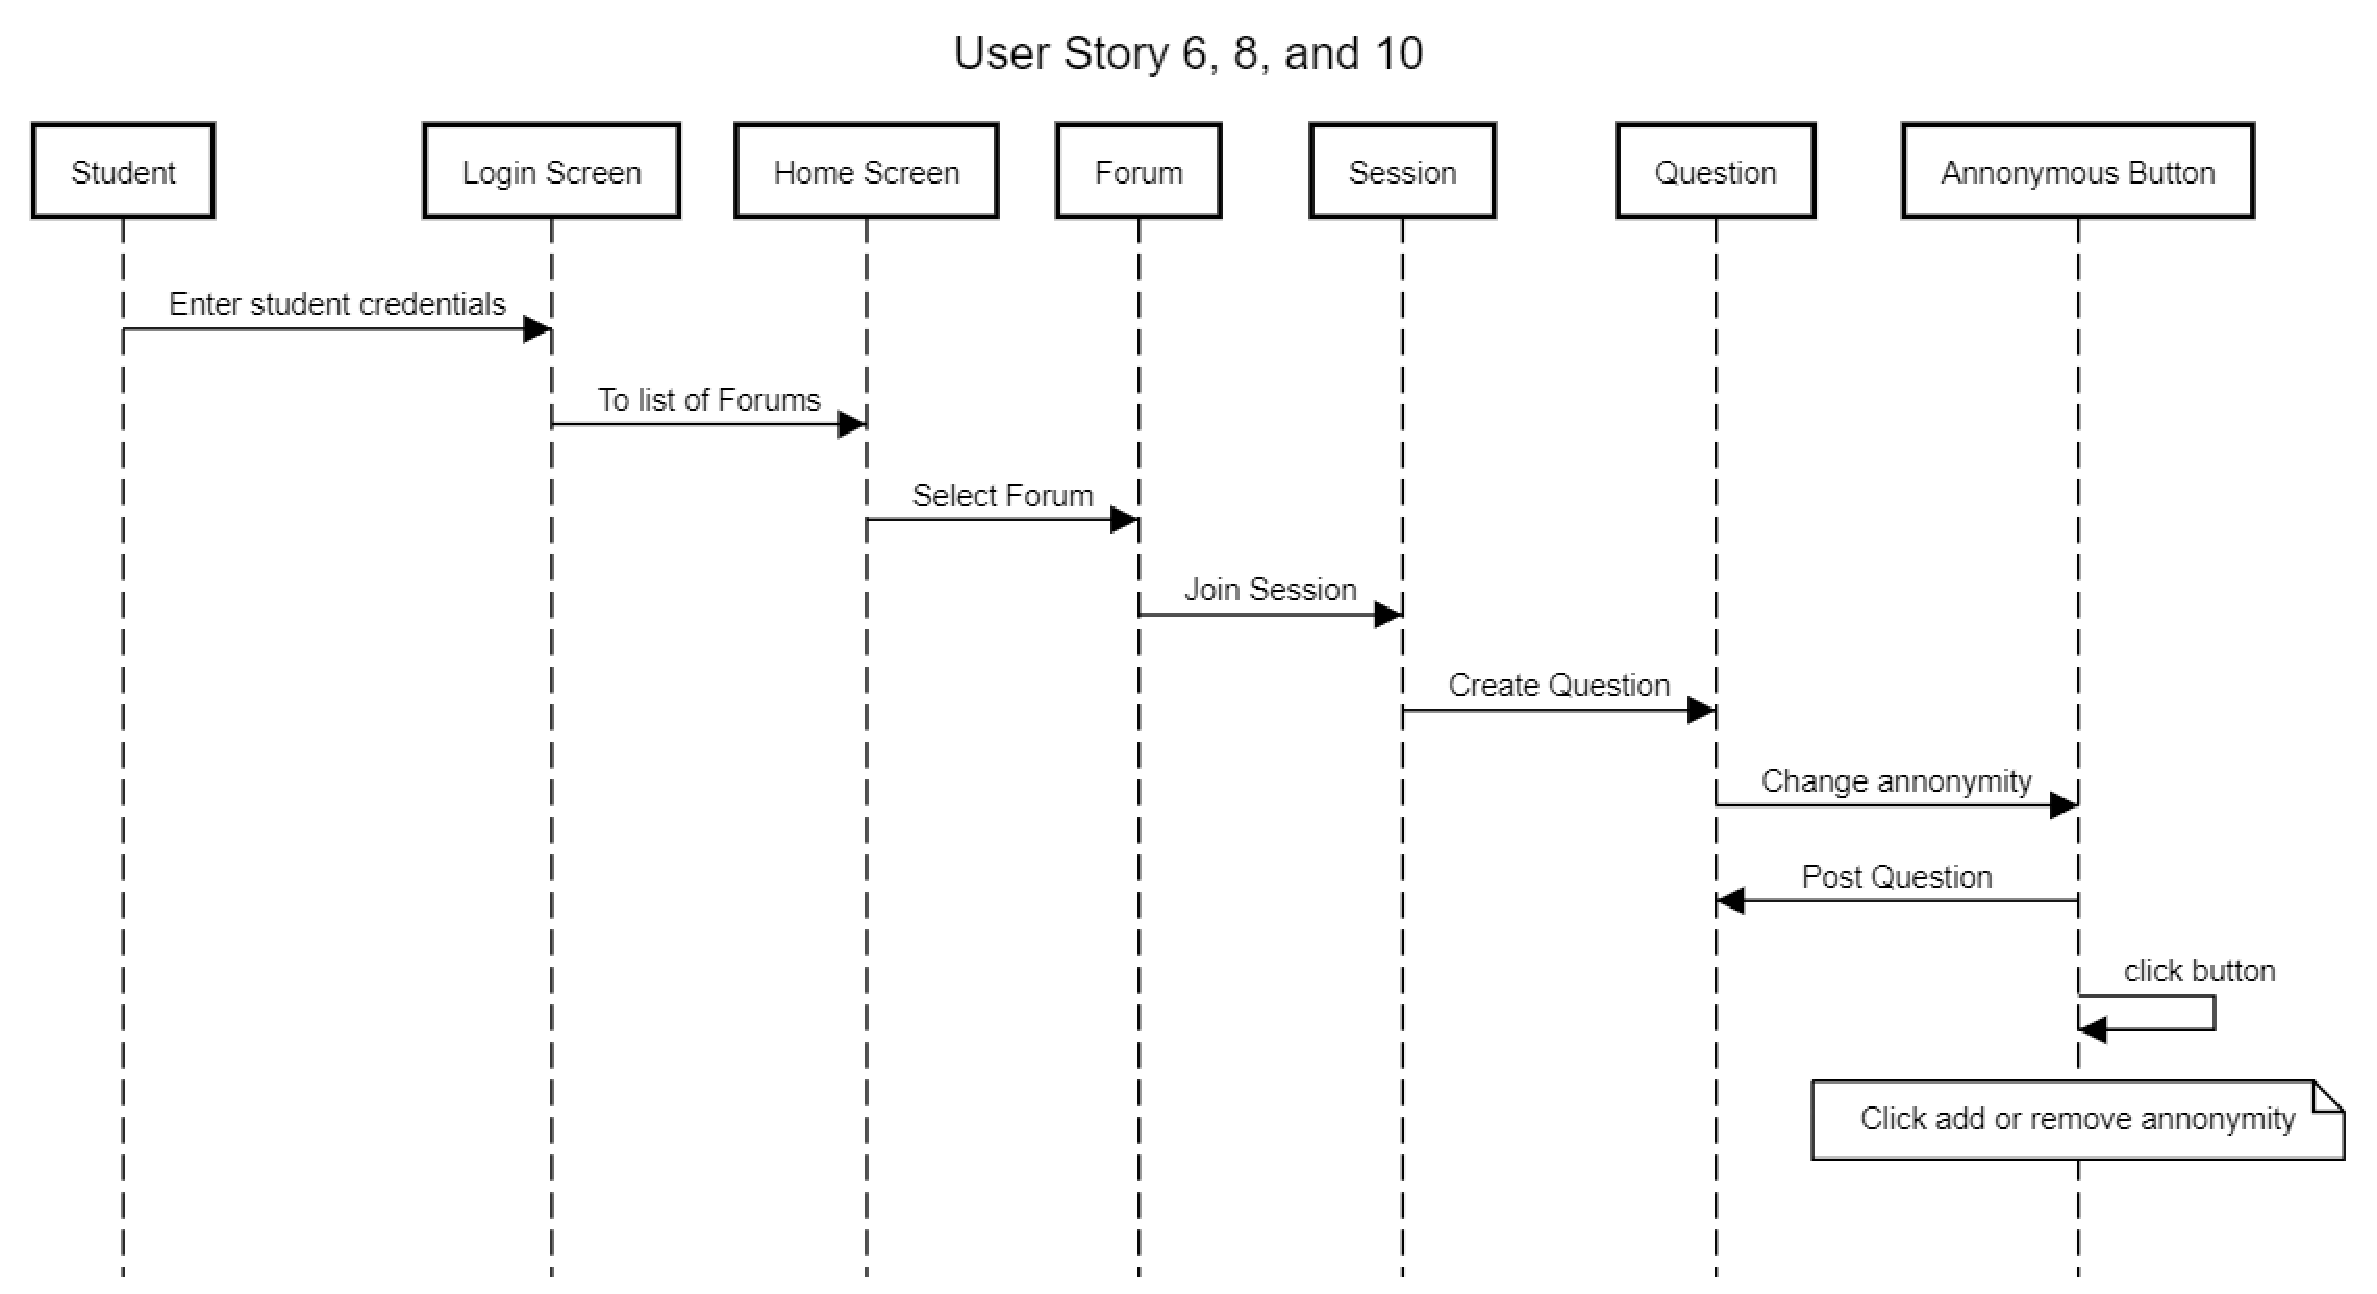
\includegraphics[width=\textwidth]{User_Story_6_8_and_10_SD.eps}
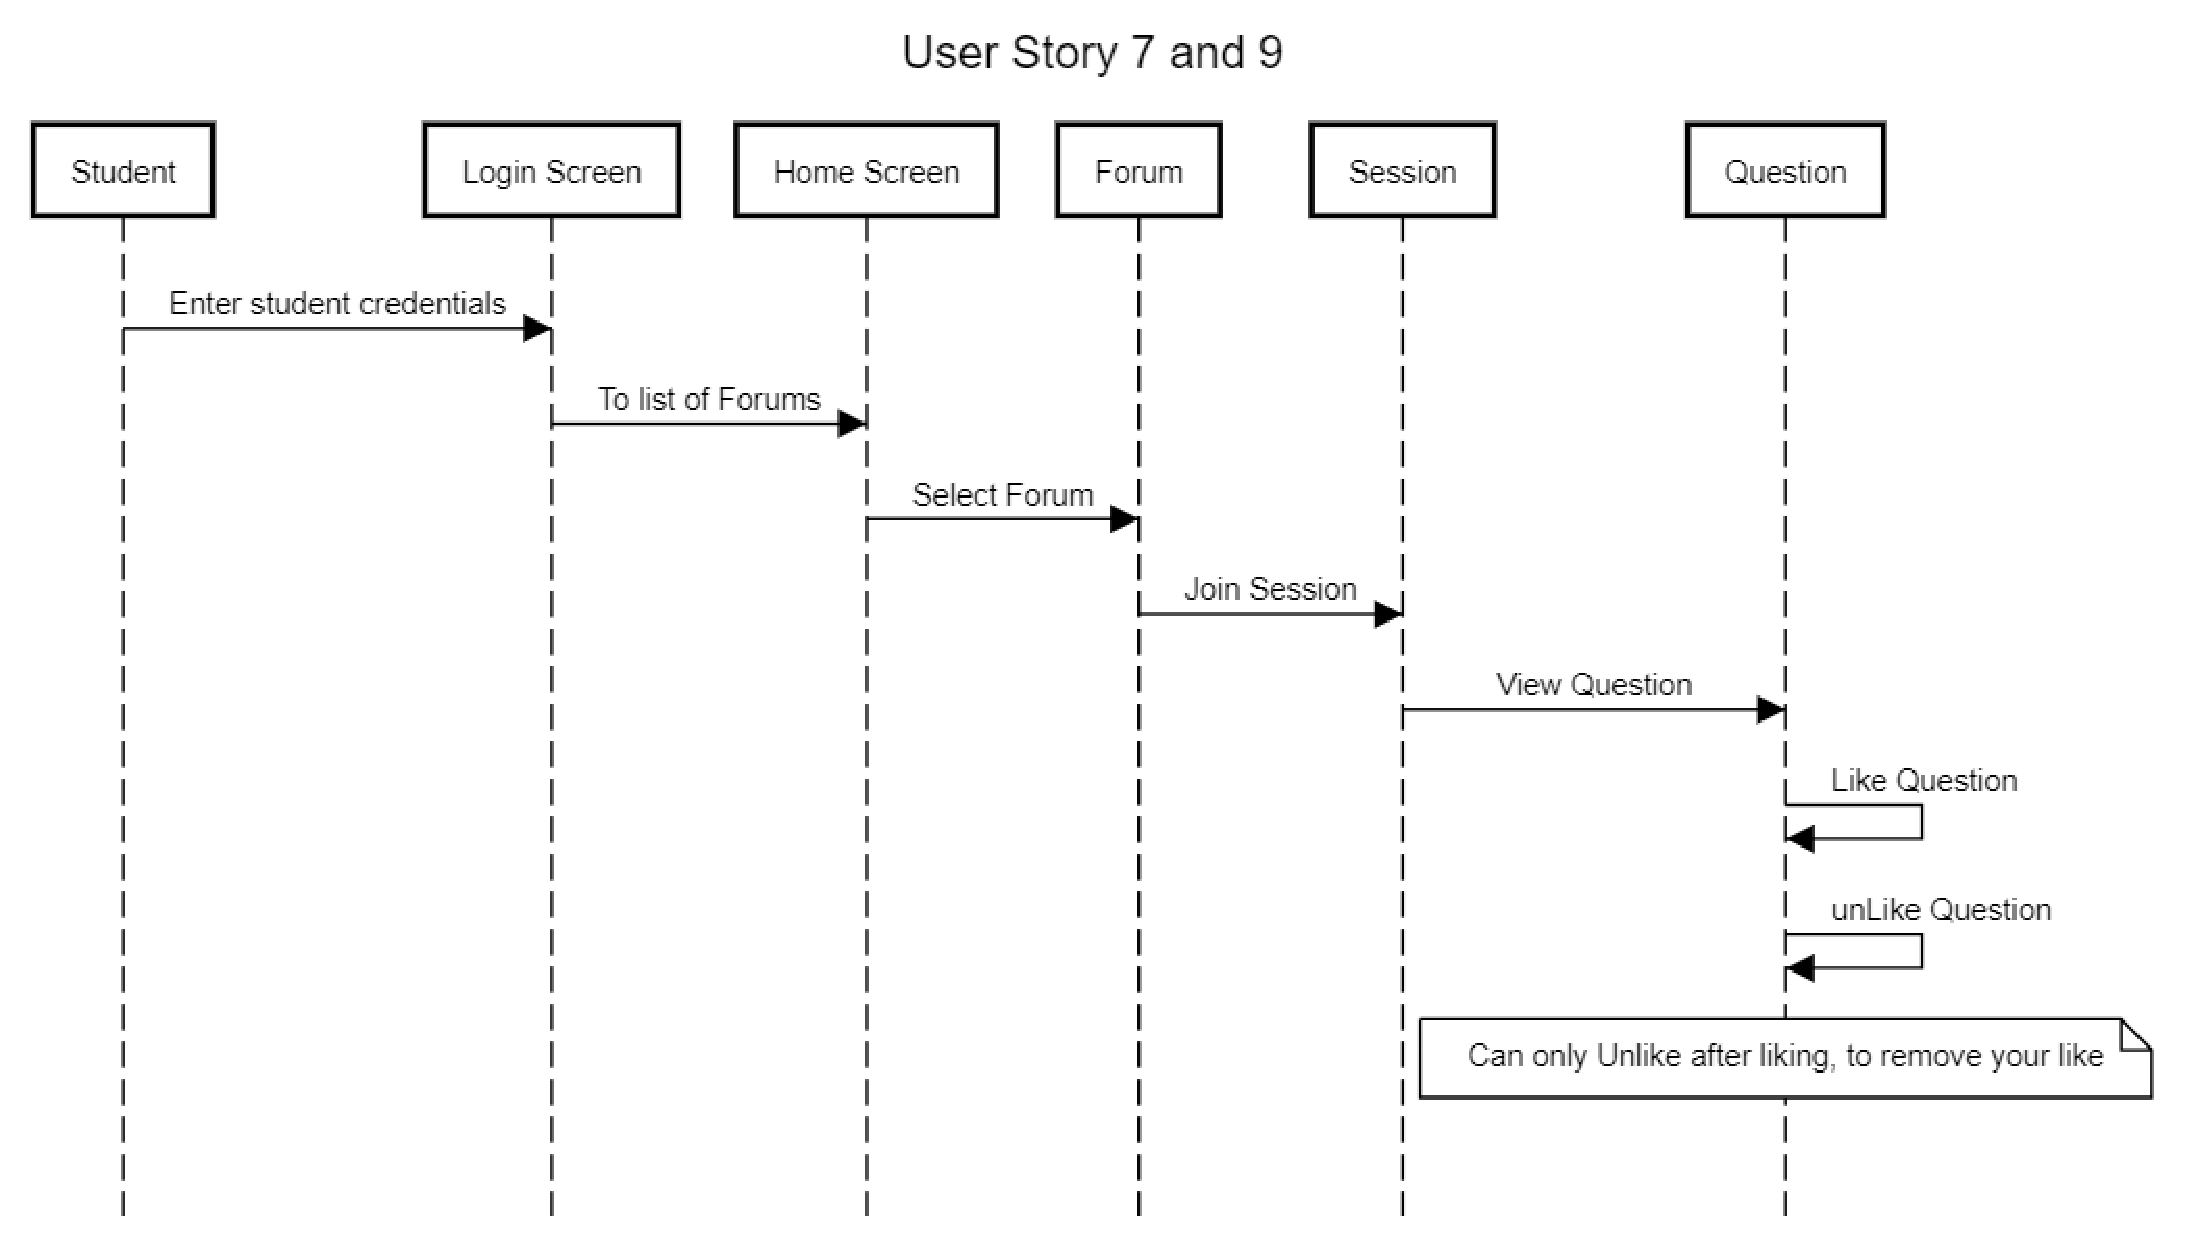
\includegraphics[width=\textwidth]{User_Story_7_and_9_SD.eps}
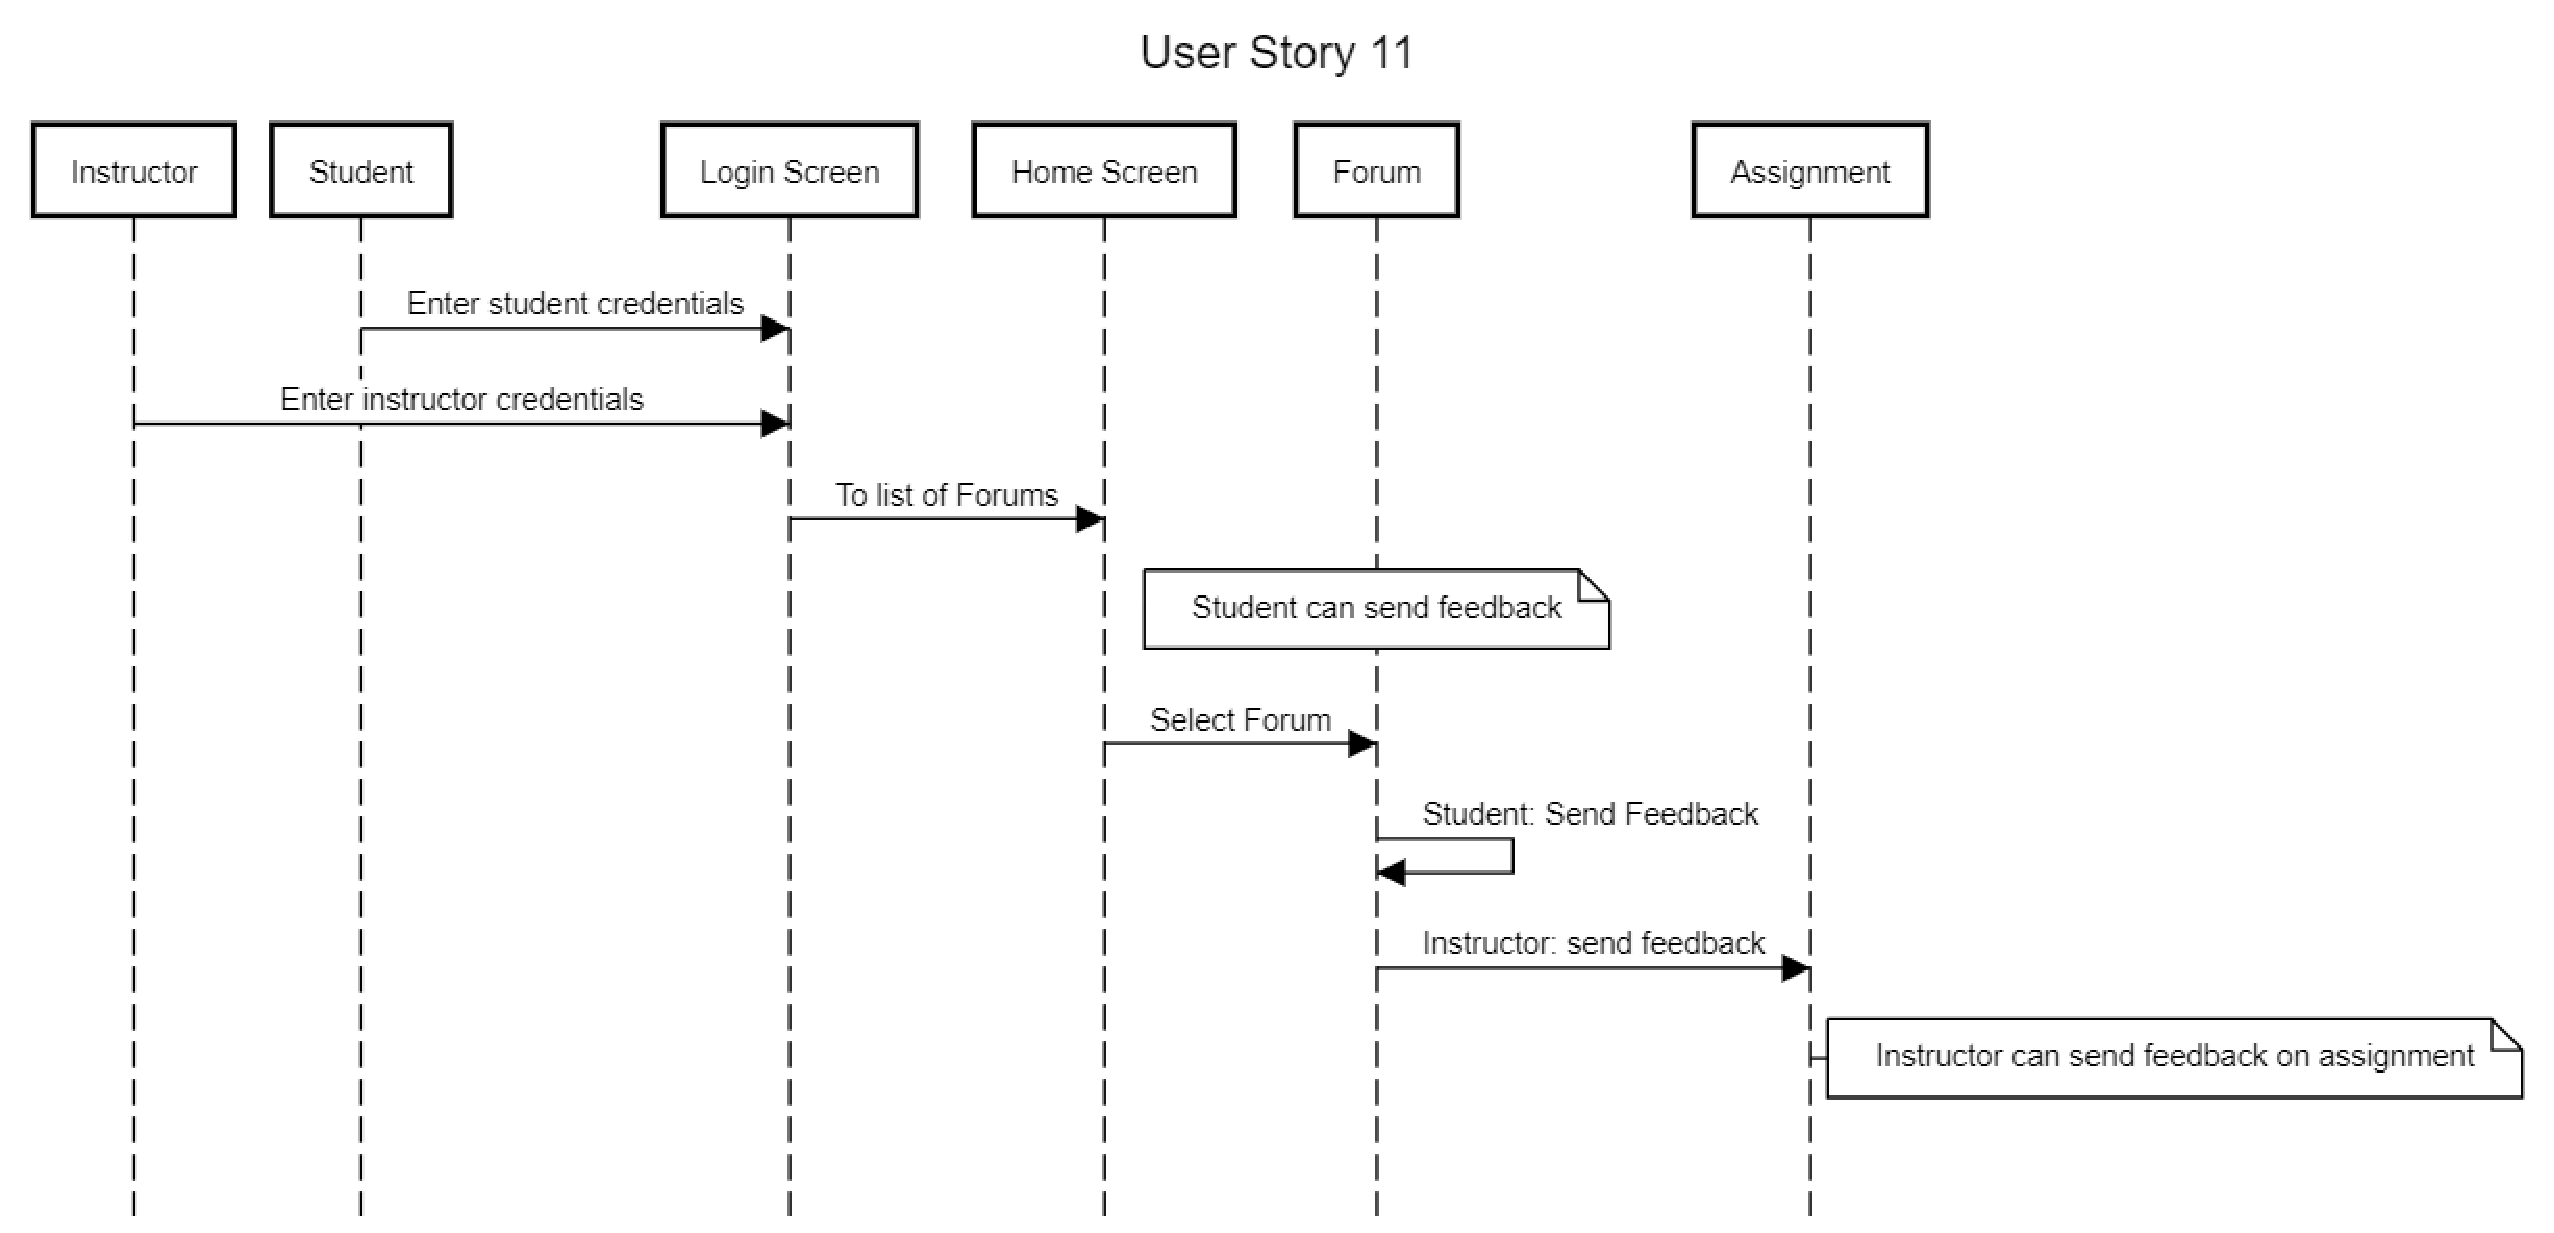
\includegraphics[width=\textwidth]{User_Story_11.eps}
\end{flushleft}


\section{Stories due Next Week}
\begin{flushleft}
Ideally, by the end of the next week we will have user stories \#1 and 2 done - that is, the base UI for our forums. This includes a login page, a signup page, a home page/landing page, forum creation, forum joining, post creation, and post reply pages. This does not mean the pages need to work! The goal for this story isn't to build the final product in one go. This is about creating the framework. Once this is built, we will be able to work on CSS (to make it look pretty) as well as database integration (for making everything work). 
\end{flushleft}
\begin{flushleft}
We will all need to work on aspects of this story at the same time; the best route would be to assign each group member a page, and split the work that way. However, there are more pages than there are people. In addition, while we shouldn't have the final CSS work done, we should have baseline formatting finished for each page. This is so we can tweak and fine-tune our product over time, as we encounter bugs or find that certain ideas don't mesh with our overall final vision. Because of all this, it's likely that we will need to split into two teams - one doing basic page creation, and the other doing basic formatting. In previous documents we've stated that one of our known weaknesses was that some team members weren't fluent in some languages. In splitting the work this way, we ensure that the group members who have experience with respective topics are doing what they know, and in addition ensure the formatting is uniform across the various parts of the Askie forum.
\end{flushleft}


\section{Meeting Report}
\begin{flushleft}
This week we were able to make significant progress in preparing to implement the program. We created a variety of user stories which assist in planning the development of the application by getting a better idea of what the customer wants from the application and how they would like it to function. The various pieces of the project are starting to come together at this point and the way in which the implementation will be completed is becoming more clear.
\end{flushleft}
\begin{flushleft}
In the next week we will begin implementing the application. We have split up the various user stories that we generated this week between us for implementation. We put a plan in place so that we can stay on track with or schedule that we have been following since the beginning. We have assigned tasks to each of this so that the work we have will be completed as efficiently as possible.
\end{flushleft}
\begin{flushleft}
In developing our plans for the next week, we had to make decisions about which tasks we can complete and which we cannot. Because of our limited schedule, we will not be able to complete all aspects of the project that the customer wants by the end of the term. Though we are not able to complete all the requirements the customer desires in the next three weeks, the customer was very understanding and worked with us to ensure we complete the most significant parts of the application. While not all of the requirements will be implemented by the deadline, we will have those requirerments implemented which will provide the customer with basic functionality. The customer understands that this is the best outcome that can be achieved by the deadline and they are supportive of our efforts.
\end{flushleft}
\end{document}
